\begin{savenotes}
    \begin{figure}
        \begin{minipage}{.5\textwidth}
            \centering
            \vspace*{-6mm}
            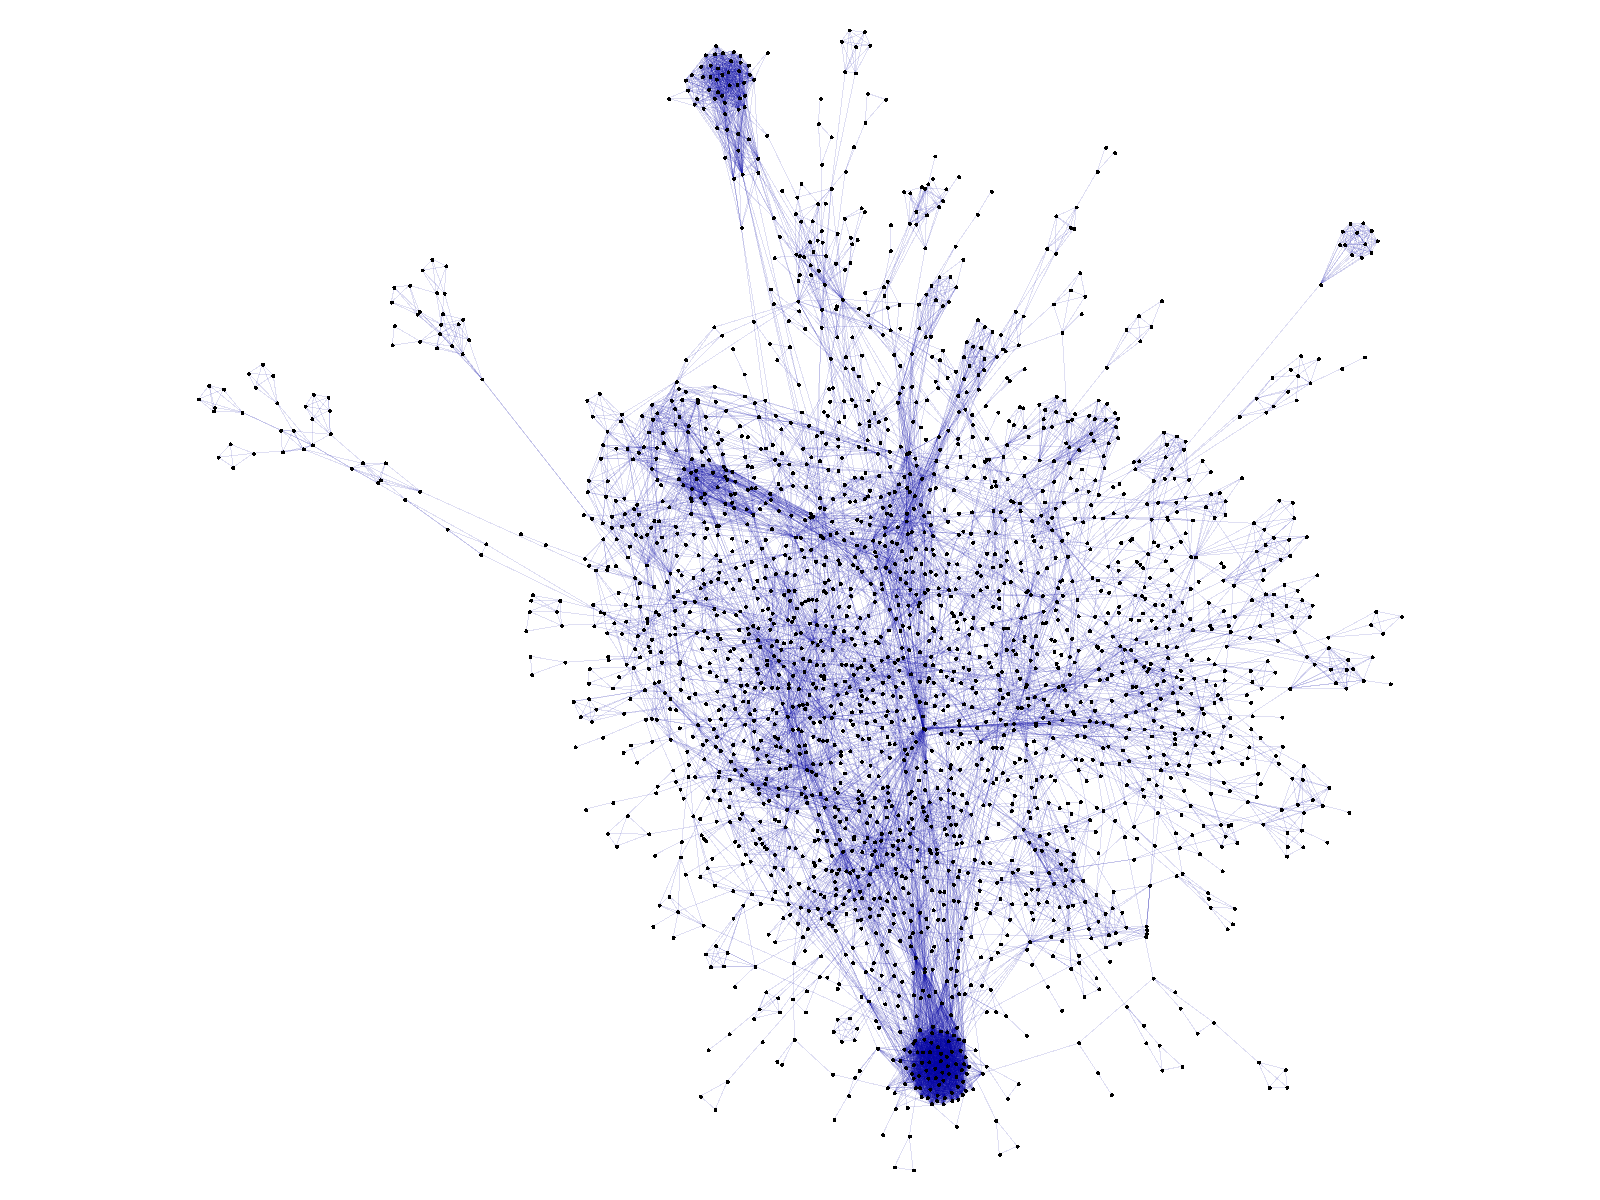
\includegraphics[width=0.85\linewidth]{ecoli_giant_at_900.png}
        \end{minipage}\hfill%
        \begin{minipage}{.5\textwidth}
            \centering
            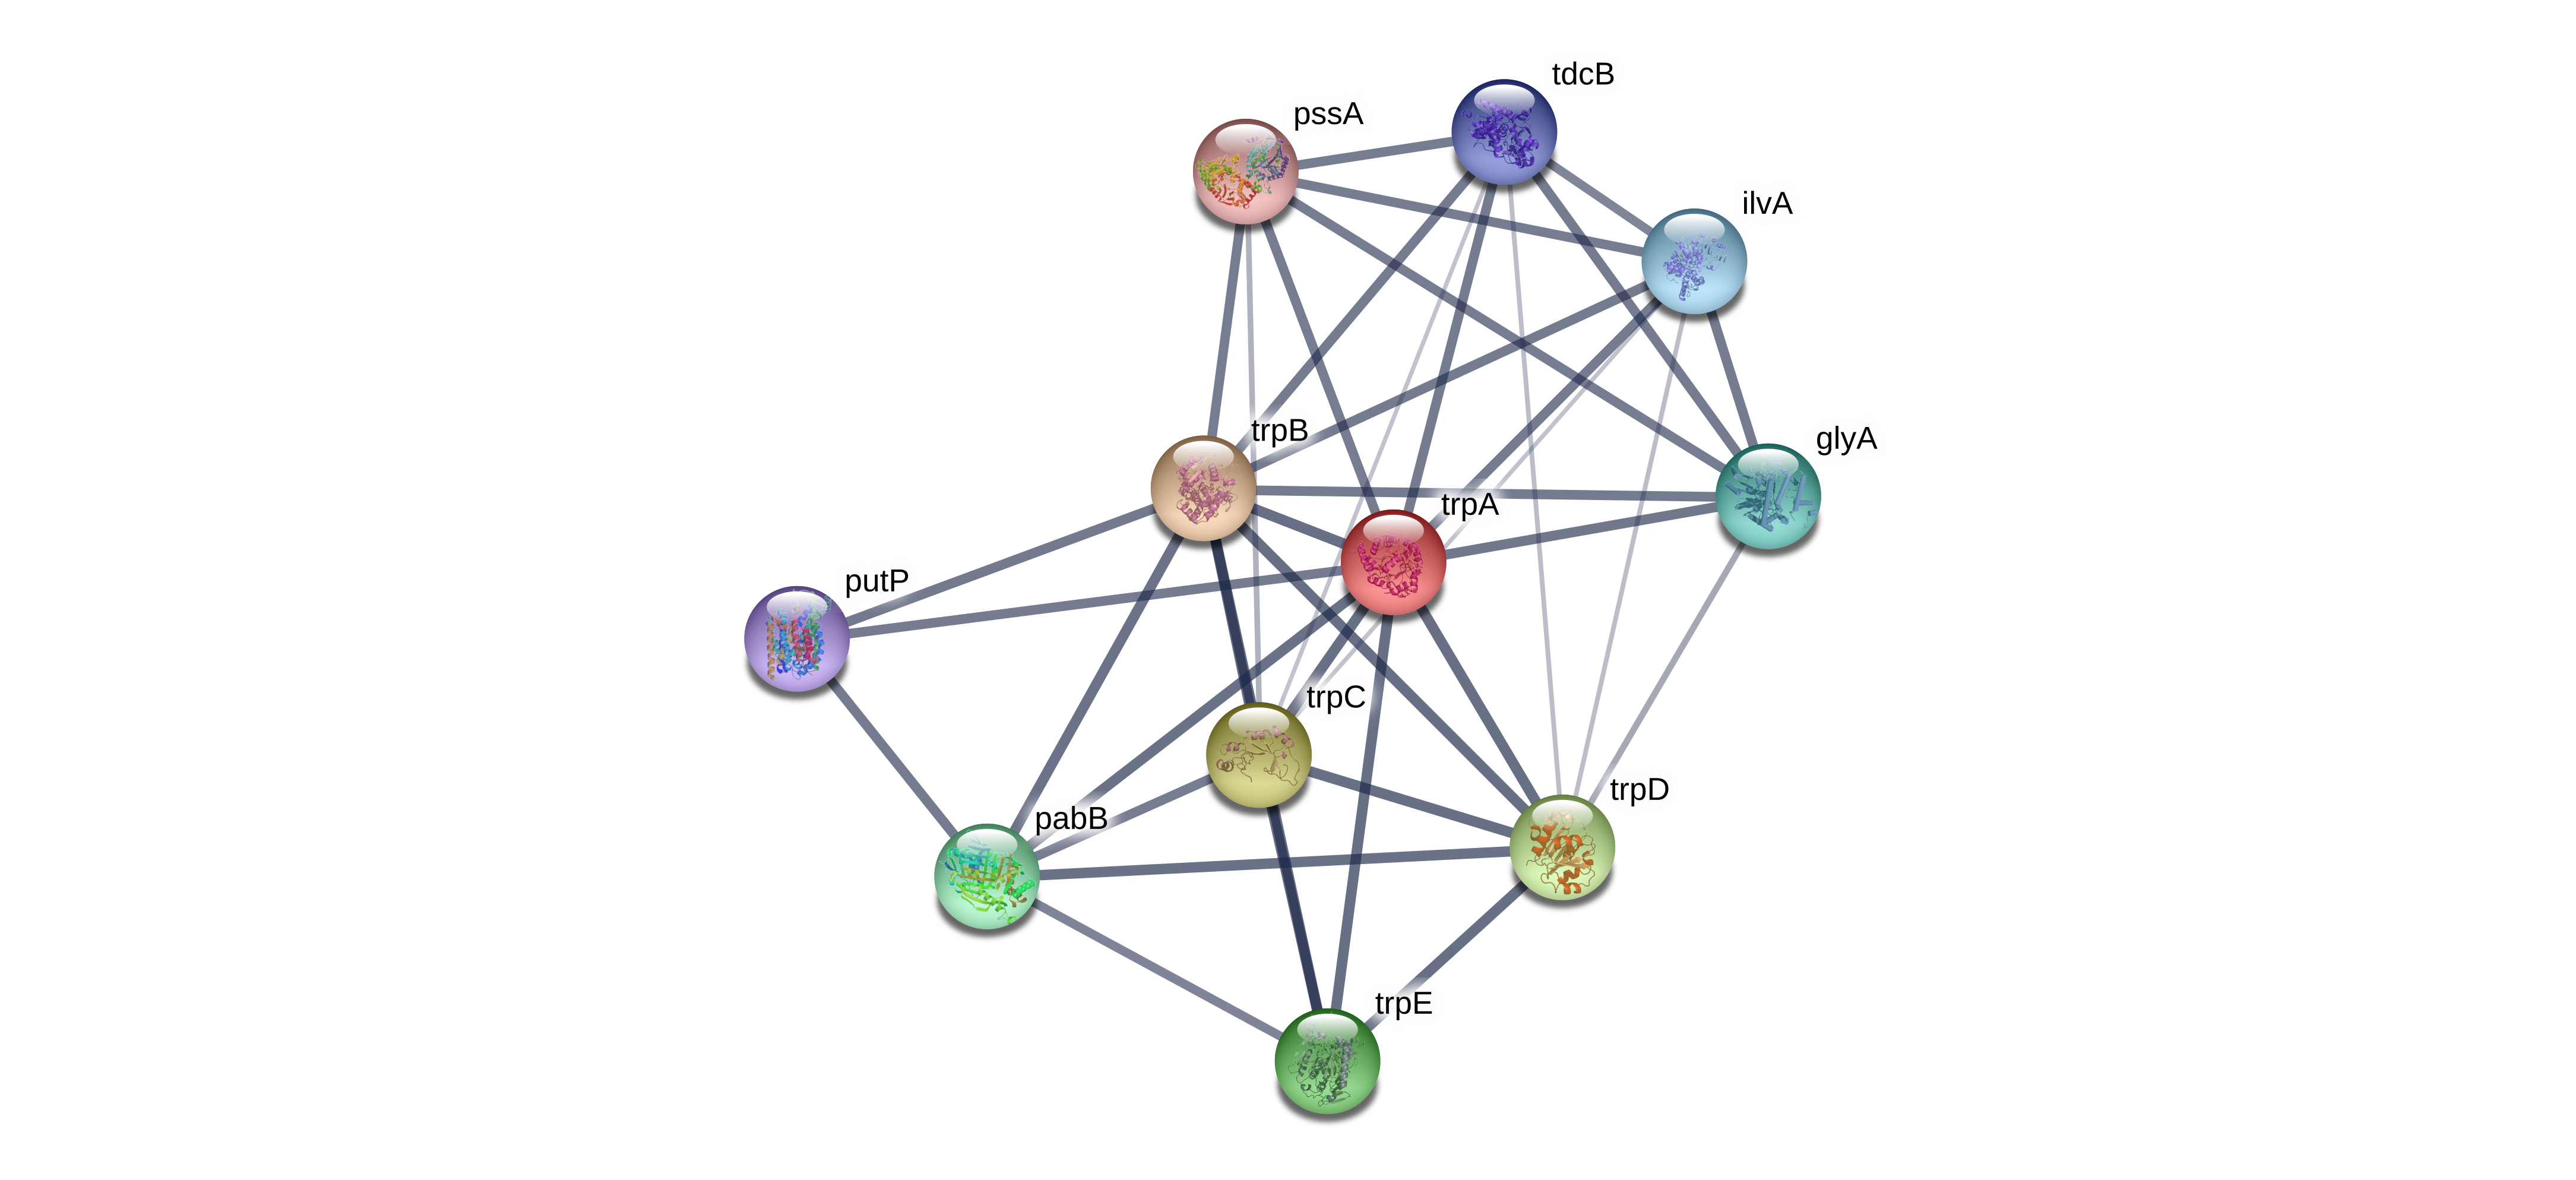
\includegraphics[width=0.55\linewidth]{string_network_image.png}
            \caption[Interactions between 11 proteins visualised by the STRING database~\cite{Szklarczyk2019}.
            Edge thickness indicates the overall confidence score, i.e. the strength of data support.]%
            {(right) Protein-protein interaction network visualised\protect\footnotemark{} by the STRING database~\cite{Szklarczyk2019}.
            Edge thickness indicates the overall confidence score, i.e. the strength of data support.}
            \footnotetext{Available at \url{https://version-11-0.string-db.org/cgi/network.pl?networkId=8lbbIYSrLfZG}}
            \label{fig:string_network_image}
        \end{minipage}
        \caption{(left) A protein interaction network from the \textit{Escherichia coli} organism from the STRING database, thresholded at the $0.9$ score (high confidence). The giant component has 2382 nodes and 12071 edges.}
        \label{fig:ecoli_giant_at_900}
    \end{figure}
\end{savenotes}
